\documentclass{standalone}
\usepackage{tikz}
\begin{document}
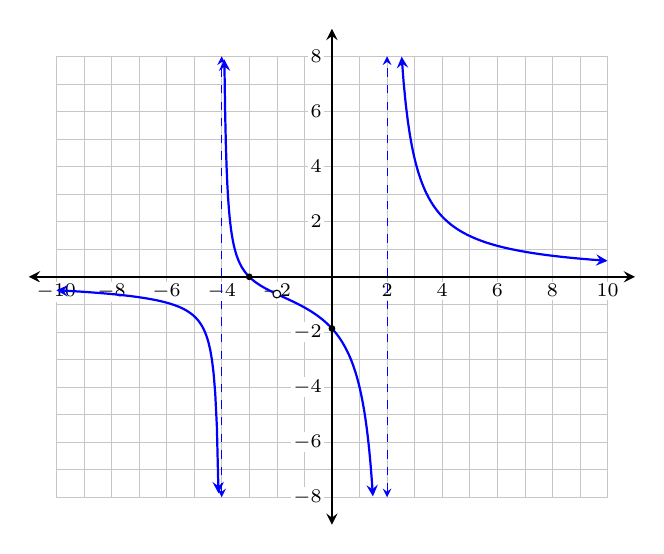
\begin{tikzpicture}[>=stealth, scale=0.35]
  % Same blank grid as 40.tex, with the graph of
  % r(x) = 5(x + 3) / ((x - 2)(x + 4)), hole at (-2, -0.625)
  \draw[gray!45, very thin] (-10,-8) grid (10,8);
  % Axes and labels drawn before the graph so the label halos
  % never hide part of the curve
  \draw[<->, thick] (-11,0) -- (11,0);
  \draw[<->, thick] (0,-9) -- (0,9);
  \foreach \x in {-10,-8,-6,-4,-2,2,4,6,8,10} {
    \node[below, font=\scriptsize, fill=white, inner sep=1pt] at (\x,-0.15) {$\x$};
  }
  \foreach \y in {-8,-6,-4,-2,2,4,6,8} {
    \node[left, font=\scriptsize, fill=white, inner sep=1pt] at (-0.25,\y) {$\y$};
  }
  % Vertical asymptotes x = -4 and x = 2 (the horizontal asymptote
  % y = 0 is the x-axis)
  \draw[<->, dashed, blue] (-4,-8) -- (-4,8);
  \draw[<->, dashed, blue] (2,-8) -- (2,8);
  % Each branch ends where the graph leaves the window (|r| = 8)
  \draw[<->, thick, blue, samples=100, domain=-10:-4.115]
    plot (\x, {5*(\x+3)/((\x-2)*(\x+4))});
  \draw[<->, thick, blue, samples=200, domain=-3.903:1.488]
    plot (\x, {5*(\x+3)/((\x-2)*(\x+4))});
  \draw[<->, thick, blue, samples=100, domain=2.530:10]
    plot (\x, {5*(\x+3)/((\x-2)*(\x+4))});
  % Zero, y-intercept, and hole
  \fill[black] (-3,0) circle (3.5pt);
  \fill[black] (0,-1.875) circle (3.5pt);
  \draw[fill=white, draw=black] (-2,-0.625) circle (4pt);
\end{tikzpicture}
\end{document}
